\documentclass[
%draft,%
twoside,%
%openleft,%
%twocolumn,%
%titlepage,%
%fleqn,%
%a4page,%
ngerman,%
headsepline%
%a4paper,%
11pt]%
{article}

% Pakete
\usepackage{fancyhdr}
\usepackage{graphicx}
\usepackage[applemac]{inputenc}
%\usepackage{german}
\usepackage{../../../../Documents/Mathematik/mymath}
\usepackage{units}
\usepackage{nicefrac}
\usepackage{pgf,tikz}
\usetikzlibrary{arrows}
\usepackage[T1]{fontenc}

%\usepackage{fancyhdr}
%\usepackage{scrpage2}
\usepackage{lastpage}
\usepackage{geometry}
\usepackage{graphicx}
\usepackage[applemac]{inputenc}
\usepackage[ngerman]{babel}
\usepackage{lscape}
%\usepackage{/Users/waj/Documents/Mathematik/mymath}
%\usepackage{units}
%\usepackage{nicefrac}
%\usepackage{pgf,tikz}
%\usetikzlibrary{arrows}
\usepackage{colortbl}
\usepackage{hhline}
\usepackage{multirow}
\usepackage[extendedchars]{grffile}
\usepackage{caption}
\usepackage{multicol,calc}
\usepackage{blindtext}
\usepackage{pdfpages}
\usepackage{hyperref}
\usepackage{wrapfig}

% Seite auf A4-Format anpassen
%\setlength{\textheight}{650pt}%
%\setlength{\voffset}{-45pt}%
%\setlength{\textwidth}{444pt}%
%\setlength{\hoffset}{-41pt}%

%Setting margins to open right my script
\let\tmp\oddsidemargin
\let\oddsidemargin\evensidemargin
\let\evensidemargin\tmp
\reversemarginpar

% Header und Footer
\pagestyle{fancy}
\fancypagestyle{myheadings}{%
\renewcommand{\footrulewidth}{0pt}
\headheight 50pt

\rhead{\hrule \ \\[1ex]
\begin{minipage}[b]{13ex}
Mathematik\\
Algebra\\
Potenzen\\
gymkl, WaJ\\[-2.5ex]
\end{minipage}
}

\chead{}%
\lhead{\Huge \textbf{\textsc{Potenzen}}\\[-1ex]}%
\rfoot{}%
\cfoot{\thepage}%
\lfoot{}%
}

\fancypagestyle{plain}{%
\headheight 30pt
\renewcommand{\headrulewidth}{0pt}
\renewcommand{\footrulewidth}{0pt}
\rhead{}%
\chead{}%
\lhead{}%
\rfoot{}%
\cfoot{}%
\lfoot{}%
}


\begin{document}
\pagestyle{myheadings}

\setcounter{page}{1}

\section{Grundbegriffe}
\begin{wrapfigure}{r}{0.318\textwidth}
  \begin{center}
    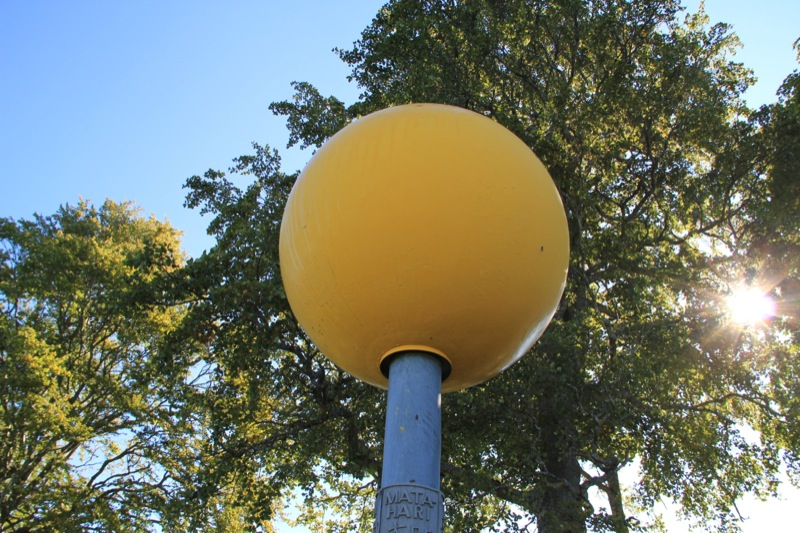
\includegraphics[width=0.318\textwidth]{sonne}
  \end{center}
%\caption{A gull}
\end{wrapfigure}
H\"aufig treten in allt\"aglichen oder wissenschaftlichen Kontexten, zum Beispiel in Physik, Biologie oder Chemie, grosse oder kleine Zahlen auf. Potenzen k\"onnen dazu verwendet werden um sehr grosse oder sehr kleine Zahlen kurz und \"ubersichtlich zu notieren. Zwei wichtige Beispiele f\"ur solche Zahlen sind folgend aufgef\"uhrt.

\begin{itemize}
\item Abstand Erde-Sonne, eine astronomische Einheit (1 AE)
$$\unit[150'000'000]{km}$$
\item Durchmesser eines Atoms, ein \AA ngstr\"om (1 \AA)
$$\unit[0.000\,000\,000\,1]{m}$$
\end{itemize}

\subsection{Potenzbegriff allgemein}
\begin{defn}
Der Term
$$a^b$$
heisst {\bf Potenz}. $a$ nennt man {\bf Basis}, $b$ heisst {\bf Exponent}.
\end{defn}

\subsection{Potenzen mit nat\"urlichen Exponenten}
\begin{defn}
F\"ur $a\in\mR$ und $n\in\mN$ soll gelten:
$$a^1=a\q\text{ und }\q a^n=\underbrace{a\cdot a\cdot a\cdot\dots\cdot a}_{\text{n Faktoren}}\text{ f\"ur }n\geq2$$
\end{defn}

\begin{bsps}
\ \\[-2ex]
\begin{itemize}
\item $2^3=2\cdot2\cdot2=8$
\item $\left(\frac{1}{3}\right)^2=\frac{1}{3}\cdot\frac{1}{3}=\frac{1}{9}$
\item $\pi^4\approx 3^4=81$
\end{itemize}
\end{bsps}

\section{Zehnerpotenzen}
Nach Definition gilt also zum Beispiel
$$10^1=10\q10^2=100\q10^3=1000$$
was leicht berechnet werden kann. Die obige Liste weist auch ein System auf: Erh\"oht man n\"amlich den Exponenten einer Zehnerpotenz um $1$, so muss man einfach die entsprechende Zahl mit $10$ multiplizieren. Wenden wir dieses Prinzip r\"uckw\"arts an, so k\"onnen wir Bedeutungen f\"ur die bislang sinnlosen Ausdr\"ucke
$$10^0\q10^{-1}\q10^{-2}\q\text{etc.}$$
festlegen. N\"amlich
$$10^0=1\q10^{-1}=0.1\q10^{-2}=0.01\q\dots$$

Lernen Sie zu den jeweiligen Zehnerpotenzen auch die entsprechenden Pr\"afixe und Ab\-k\"ur\-zungen, vielleicht mit Tabelle \ref{tab:zehnerpotenzen} auf Seite \pageref{tab:zehnerpotenzen}. Sie geh\"oren einer umfassenden Allgemeinbildung, da sie uns im Alltag begegnen. Damit l\"asst sich leicht erkl\"aren, wie viel ein Milliliter ist, was man unter einer Dekade versteht, wie viele Bytes ein Terabyte sind oder was unter den Begriff Mikrokosmos f\"allt. Auch eine namhafte Firma scheut sich nicht davor, ihr Flaggschiff i*** Nano zu nennen, um zu suggerieren, dass \dots.

\begin{table}
\begin{center}
\scalebox{0.9}{
  \begin{tabular}[ht]{lrlll}
    \rule[-3mm]{0mm}{24pt}
    $10^{12}\qq$ & $1\,000\,000\,000\,000$ & $\qq\qq\qq1$ Billion & \hspace*{1cm}Tera- & T\\
    \rule[-3mm]{0mm}{24pt}
    $10^{11}\qq$ & $100\,000\,000\,000$ &  &  & \\
    \rule[-3mm]{0mm}{24pt}
    $10^{10}\qq$ & $10\,000\,000\,000$ &  &  & \\
    \rule[-3mm]{0mm}{24pt}
    $10^{9}\qq$ & $1\,000\,000\,000$ & $\qq\qq\qq1$ Milliarde & \hspace*{1cm}Giga- & G\\
    \rule[-3mm]{0mm}{24pt}
    $10^{8}\qq$ & $100\,000\,000$ &  &  & \\
    \rule[-3mm]{0mm}{24pt}
    $10^{7}\qq$ & $10\,000\,000$ &  &  & \\
    \rule[-3mm]{0mm}{24pt}
    $10^{6}\qq$ & $1\,000\,000$ & $\qq\qq\qq1$ Million & \hspace*{1cm}Mega- & M\\
    \rule[-3mm]{0mm}{24pt}
    $10^{5}\qq$ & $100\,000$ &  &  & \\
    \rule[-3mm]{0mm}{24pt}
    $10^{4}\qq$ & $10\,000$ &  &  & \\
    \rule[-3mm]{0mm}{24pt}
    $10^{3}\qq$ & $1\,000$ & $\qq\qq\qq1$ Tausend & \hspace*{1cm}Kilo- & k\\
    \rule[-3mm]{0mm}{24pt}
    $10^{2}\qq$ & $100$ &  & \hspace*{1cm}Hekto- & h\\
    \rule[-3mm]{0mm}{24pt}
    $10^{1}\qq$ & $10$ &  & \hspace*{1cm}Deka- & d\\
    \rule[-3mm]{0mm}{24pt}
    $10^{0}\qq$ & $1$ &  &  & \\
    \rule[-3mm]{0mm}{24pt}
    $10^{-1}\qq$ & $0.1$ &  & \hspace*{1cm}Dezi- & d\\
    \rule[-3mm]{0mm}{24pt}
    $10^{-2}\qq$ & $0.01$ &  & \hspace*{1cm}Centi- & c\\
    \rule[-3mm]{0mm}{24pt}
    $10^{-3}\qq$ & $0.001$ & $\qq\qq\qq1$ Tausendstel & \hspace*{1cm}Milli- & m\\
    \rule[-3mm]{0mm}{24pt}
    $10^{-4}\qq$ & $0.000\,1$ &  &  & \\
    \rule[-3mm]{0mm}{24pt}
    $10^{-5}\qq$ & $0.000\,01$ &  &  & \\
    \rule[-3mm]{0mm}{24pt}
    $10^{-6}\qq$ & $0.000\,001$ & $\qq\qq\qq1$ Millionstel & \hspace*{1cm}Mikro- & $\mu$\\
    \rule[-3mm]{0mm}{24pt}
    $10^{-7}\qq$ & $0.000\,000\,1$ &  &  & \\
    \rule[-3mm]{0mm}{24pt}
    $10^{-8}\qq$ & $0.000\,000\,01$ &  &  & \\
    \rule[-3mm]{0mm}{24pt}
    $10^{-9}\qq$ & $0.000\,000\,001$ & $\qq\qq\qq1$ Milliardstel & \hspace*{1cm}Nano- & n\\
    \rule[-3mm]{0mm}{24pt}
    $10^{-10}\qq$ & $0.000\,000\,000\,1$ &  &  & \\
    \rule[-3mm]{0mm}{24pt}
    $10^{-11}\qq$ & $0.000\,000\,000\,01$ &  &  & \\
    \rule[-3mm]{0mm}{24pt}
    $10^{-12}\qq$ & $0.000\,000\,000\,001$ & $\qq\qq\qq1$ Billionstel & \hspace*{1cm}Piko & p\\
  \end{tabular}
  }
    \end{center}
    \caption{Zehnerpotenzen: Namen und Abk\"urzungen}\label{tab:zehnerpotenzen}
 \end{table}

\section{Wissenschaftliche Darstellung}
\subsection{Begriff}
Wir kommen auf unsere Motivation zu Beginn des Kapitels zur\"uck; der schlanken Darstellung grosser und kleiner Zahlen. Bei der sogenannten \emph{wissenschaftlichen Darstellung} von Zahlen schreibt man die Zahl als Dezimalbruch mit Einer und Zehnerpotenzen.
\begin{bsps}
\ \\[-2ex]
\begin{itemize}
\item Abstand Erde-Sonne, eine astronomische Einheit (1 AE)
$$\unit[150'000'000]{km}=\unit[1.5\cdot10^8]{km}$$
\item Durchmesser eines Atoms, ein \AA ngstr\"om (1 \AA)
$$\unit[0.000\,000\,000\,1]{m}=\unit[1\cdot10^{-10}]{m}$$
\item $$92'300=9.23\cdot10^4$$
\item $$0.0032=3.2\cdot10^{-3}$$
\end{itemize}
\end{bsps}

\begin{bem}
Man findet leicht eine Merkregel, um den jeweiligen Wert des Exponenten zur Basis $10$ zu bestimmen.
\end{bem}

\subsection{†bungen zur wissenschaftlichen Schreibweise}

\begin{ueb}[expand]
  Schreibe die Zahlen aus:
  \\[2.5ex]\hspace*{2.7ex}
  \begin{minipage}{0.4\textwidth}
    \begin{enumeratea}
      \item $2.52\cdot10^{5}$
      \item $6.52\cdot10^{7}$
      \item $5.555\cdot10^{12}$
      \item $4.15\cdot10^{9}$\\[1ex]
    \end{enumeratea}
  \end{minipage}
  \begin{minipage}{0.23\textwidth}
    \begin{enumeratea}\addtocounter{enumi}{4}
      \item $4.31\cdot10^{9}$
      \item $3.11\cdot10^{3}$
      \item $1.23\cdot10^{6}$
      \item $6.22\cdot10^{4}$\\[1ex]
    \end{enumeratea}
  \end{minipage}
\end{ueb}

\begin{ueb}[factor]
  Schreibe in wissenschaftlicher Darstellung:
  \\[2.5ex]\hspace*{2.7ex}
  \begin{minipage}{0.4\textwidth}
    \begin{enumeratea}
      \item $99'000'000$
      \item $4'180'000'000$
      \item $48'500'000$
      \item $0.000\,008\,21$
      \item $92'400$
      \item $0.000\,016$\\[1ex]
    \end{enumeratea}
  \end{minipage}
  \begin{minipage}{0.23\textwidth}
    \begin{enumeratea}\addtocounter{enumi}{6}
      \item $19'300$
      \item $2'340$
      \item $1'350'000$
      \item $0.000\,000\,000\,101$
      \item $822'000'000$
      \item $0.000\,000\,077$\\[1ex]
    \end{enumeratea}
  \end{minipage}
\end{ueb}


\begin{ueb}[sci]
  Schreibe in wissenschaftlicher Darstellung:
  \\[2.5ex]\hspace*{2.7ex}
  \begin{minipage}{0.4\textwidth}
    \begin{enumeratea}
      \item $0.000\,015$
      \item $0.000\,008\,1$
      \item $0.654$
      \item $0.000\,000\,074$\\[1ex]
    \end{enumeratea}
  \end{minipage}
  \begin{minipage}{0.23\textwidth}
    \begin{enumeratea}\addtocounter{enumi}{4}
      \item $0.000\,000\,25$
      \item $0.000\,005\,15$
      \item $0.000\,000\,061\,5$
      \item $0.000\,000\,000\,077$\\[1ex]
    \end{enumeratea}
  \end{minipage}
\end{ueb}

\begin{ueb}[float]
  Schreibe die Zahlen aus:
  \\[2.5ex]\hspace*{2.7ex}
  \begin{minipage}{0.4\textwidth}
    \begin{enumeratea}
      \item $1.25\cdot10^{-5}$
      \item $7.22\cdot10^{-7}$
      \item $3.33\cdot10^{-12}$
      \item $4.15\cdot10^{-4}$
      \item $8.76\cdot10^{-3}$
      \item $3.92\cdot10^{-9}$\\[1ex]
    \end{enumeratea}
  \end{minipage}
  \begin{minipage}{0.23\textwidth}
    \begin{enumeratea}\addtocounter{enumi}{6}
      \item $2.31\cdot10^{-9}$
      \item $2.75\cdot10^{-5}$
      \item $5.05\cdot10^{-6}$
      \item $6.02\cdot10^{-8}$
      \item $7.07\cdot10^{-7}$
      \item $6.1\cdot10^{-6}$\\[1ex]
    \end{enumeratea}
  \end{minipage}
\end{ueb}

\section{Rechenregeln f\"ur Potenzen}
Insbesondere beim Rechnen mit Variablen aber auch f\"urs Kopfrechnen k\"onnen folgende Regeln zu Hilfe genommen werden.

\subsection{Erinnerung}
Wir erinnern uns an die Definition der Potenz f\"ur nat\"urliche Exponenten.

\begin{defn}
F\"ur $a\in\mR$ und $n\in\mN$ soll gelten:
$$a^1=a\q\text{ und }\q a^n=\underbrace{a\cdot a\cdot a\cdot\dots\cdot a}_{\text{n Faktoren}}\text{ f\"ur }n\geq2$$
\end{defn}

Damit lassen sich leicht die folgenden Potenzgesetze einsehen.

\subsection{Potenzgesetze}
F\"ur die folgenden Ausf\"uhrungen seien $a,b\in\mR$ und $m,n\in\mN$; sowie bei Bedarf $n>m$. Es gilt
\begin{align}
a^n\cdot a^m&=a^{n+m}\\
a^n\div a^m&=a^{n-m}\\
\left(a^n\right)^m&=a^{n\cdot m}\\
a^n\cdot b^n&=(a\cdot b)^{n}\\
a^n\div b^n&=(a\div b)^{n}
\end{align}
\begin{bem}
Die ersten beiden Gesetze beziehen sich auf Potenzen mit denselben Basen, die letzten beiden auf Potenzen mit gleichen Exponenten.
\end{bem}

\begin{bsps}
Folgend je ein Anwendungsbeispiel zu jedem Gesetz:
\begin{itemize}
\item $x^{2n}\cdot x^{3-n}=x^{2n+3-n}=x^n+3$
\item $z^7\div z^{3-n}=z^{7-(3-n)}=z^{n+4}$
\item $\left(2^3\right)^4=2^{3\cdot4}=2^{12}=4096$
\item $2^4\cdot5^4=(2\cdot5)^4=10^4=10000$
\item $25^3\div5^3=(25\div5)^3=5^3=125$
\end{itemize}
\end{bsps}

\section{Das Pascal'sche Dreieck}
\subsection{Einleitung}
\begin{ueb}
Multipliziere aus.
  \\[2.5ex]\hspace*{2.7ex}
  \begin{minipage}{0.4\textwidth}
    \begin{enumeratea}
      \item $(a+b)^1$
      \item $(a+b)^2$\\[1ex]
    \end{enumeratea}
  \end{minipage}
  \begin{minipage}{0.23\textwidth}
    \begin{enumeratea}\addtocounter{enumi}{2}
      \item $(a+b)^3$
      \item $(a+b)^7$\\[1ex]
    \end{enumeratea}
  \end{minipage}
  \end{ueb}
  
Die †bungen (a) und (b) gehen leicht von der Hand. Teil\"ubung (c) bedarf schon etwas mehr Aufwand und (d) scheint unmenschlich. Aber, beim Ausmultiplizieren von potenzierten Summen, insbesondere von \emph{\"ublen} Summen wie $(a+b)^6$, kann das Pascal'sche Dreieck n\"utzlich sein; dazu sp\"ater. Im Folgenden sollen nun das Pascal-Dreieck und einige seiner Eigenschaften pr\"asentiert werden.
\subsection{Aufbau}
Das Pascal'sche Dreieck sieht wie folgt aus; es kann theoretisch unendlich \glqq hoch\grqq\ werden.

  \begin{center}
    \ \\[2pt]
    $1$\\[6pt]
    $1\qq1$\\[6pt]
    $1\qq2\qq1$\\[6pt]
    $1\qq3\qq3\qq1$\\[6pt]
    $1\qq4\qq6\qq4\qq1$\\[6pt]
    $1\qq5\qq10\qq10\qq5\qq1$\\[6pt]
    $1\qq6\qq15\qq20\qq15\qq6\qq1$\\[6pt]
    $1\qq7\qq21\qq35\qq35\qq21\qq7\qq1$\\[6pt]
    $\dots$
  \end{center}

\begin{frage}
Beschreibe Regeln f\"ur die Konstruktion des Pascal-Dreiecks?
\end{frage}
Offensichtlich besteht das Dreieck aus lauter $1$-en am Rand. In jeder folgenden Zeile nimmt die Anzahl der Zahlen um Eins zu. Die Zahl in der unteren Zeile ist gleich der Summe der dar\"uber liegenden Zahlen. Theoretisch kann man die $k$-te Zahl in der $n$-ten Zeile auch direkt berechnen  --- dabei beginnt man die Zeilen mit $0$ durchzunummerieren. Die Zugrunde liegende Formel ist allerdings nicht leicht zu finden.

\begin{frage}
Welche Eigenschaften erkennt man?
\end{frage}

\subsection{Eigenschaften}
Das Pascal-Dreieck besitzt unter anderem folgende Eigenschaften
\begin{itemize}
\item In der Diagonalen $1,3,6,10,15,\dots$ liest man die Dreieckszahlen ab.
\item Die Summe der $n$-ten Zeile entspricht der Zweierpotenz $2^{n}$.
\item Das Verh\"altnis zweier benachbarter Zahlen einer Zeile entspricht dem Verh\"altnis der Anzahl Zahlen, die links und rechts davon stehen inklusive.
\end{itemize}

\noindent Pascal formulierte die letzte Eigenschaft wie folgt:
\begin{quote}
  \glqq En tout triangle arithmŽtique, deux cellules contigu‘s Žtant dans
  une mme base, la supŽrieure est ˆ l'infŽrieure comme la multitude
  des cellules depuis la supŽrieure jusqu'au haut de la base ˆ la
  multitude de cellules depuis l'infŽrieure jusqu'en bas
  inclusivement.\grqq
\end{quote}

Die f\"ur unser Anfangsproblem wichtigste Eigenschaft ist

\begin{itemize}
\item Die Zahlen in der $n$-ten Zeile sind die Koeffizienten der Summanden des ausmultiplizierten Terms $(a+b)^n$.
\end{itemize}

  \begin{align}
    (a+b)^0 &= 1\notag\\
    (a+b)^1 &= a+b\notag\\
    (a+b)^2 &= a^2+2ab+b^2\notag\\
    (a+b)^3 &= a^3+3a^2b+3ab^2+b^3\notag\\
    (a+b)^4 &= a^4+4a^3b+6a^2b^2+4ab^3+b^4\notag\\
    \dots &\dots\notag
  \end{align}

  \begin{center}
    \ \\[2pt]
    $1$\\[6pt]
    $1\qq1$\\[6pt]
    $1\qq2\qq1$\\[6pt]
    $1\qq3\qq3\qq1$\\[6pt]
    $1\qq4\qq6\qq4\qq1$\\[6pt]
    $\dots$
  \end{center}

Diese Eigenschaft erlaubt uns also, Terme der Form $(a+b)^n$ ohne grossen Rechenaufwand ausmultiplizieren zu k\"onnen.
\begin{bem}
Das Pascal-Dreieck liefert uns die Koeffizienten des ausmultiplizierten Terms. Weiter gilt f\"ur die beteiligten Summanden $a$ und $b$, dass die Exponenten von $a$ mit dem gr\"ossten Wert des Exponenten starten und bei jedem weiteren Summanden um $1$ abnehmen; f\"ur den Summanden $b$ ist das Gegenteil der Fall: er taucht beim ersten Summanden nicht auf, dann als $b=b^1$, danach als $b^2$, etc.
\end{bem}
\begin{bsp}
$$(a+b)^3=a^3+3a^2b+3ab^2+b^3$$
\end{bsp}
Wendet man nun diese Strategie auf \"ahnliche Terme an, so sind $a$ und $b$ bloss durch die entsprechenden Summanden zu ersetzen.
\begin{bsp}
F\"ur $(z^2-2b)^3$ ist $a=z^2$ und $b=-2b$. Also
\begin{align*}
(z^2-2b)^3&=(z^2)^3+3\cdot(z^2)^2\cdot(-2b)+\\
&\phantom{=\;}+3\cdot(z^2)\cdot(-2b)^2+(-2b)^3\\
&=z^6-6z^4b+12z^2b^2-8b^3
\end{align*}
\end{bsp}

\begin{ueb}
Berechne mit Hilfe des Pascal'schen Dreieck

\begin{minipage}{0.23\textwidth}
\begin{enumeratea}
\item $(x-1)^5$
\item $(-3+2c)^3$
\end{enumeratea}
\end{minipage}
\begin{minipage}{0.23\textwidth}
\begin{enumeratea}
\addtocounter{enumi}{2}
\item $(y^3-2)^3$
\item $(x+2y+z)^4$
\end{enumeratea}
\end{minipage}
\end{ueb}

\pagebreak

\section*{L\"osungen}

\hspace*{2.7ex} 1.) $252\,000; 65\,200\,000; 5\,555\,000\,000\,000;4\,150\,000\,000;4\,310\,000\,000;3110;1\,230\,000;62\,200.$

2.) $9.9\cdot10^{7};4.18\cdot10^{9};4.85\cdot10^{7}; 8.21\cdot10^{-6}; 9.24\cdot10^{4}; 1.6\cdot10^{-5}; 1.93\cdot10^{4}; 2.34\cdot10^{3}; 1.35\cdot10^{6}$;
\hspace*{7ex}$1.01\cdot10^{-10}; 8.22\cdot10^{8}; 7.7\cdot10^{-8}.$

3.) $1.5\cdot10^{-5};8.1\cdot10^{-6}; 6.54\cdot10^{-1}; 7.4\cdot10^{-8}; 2.5\cdot10^{-7}; 5.15\cdot10^{-6}; 6.15\cdot10^{-8}; 7.7\cdot10^{-11}.$

4.) $0.0000125; 0.000000722; 0.00000000000333; 0.000415; 0.00876; 0.00000000392; 0.00000000231;$
\hspace*{7ex}$0.0000275; 0.00000505; 0.0000000602; 0.000000707; 0.0000061.$

5.) $a+b; a^2+2ab+b^2; a^3+3a^2b+3ab^2+b^3; a^7+7a^6b+21a^5b^2+35a^4b^3+35a^3b^4+21a^2b^5+7ab^6+b^7.$

6.) $x^5-5x^4+10x^3-10x^2+5x-1; -27+54c-36c^2+8c^3; y^9-6y^6+12y^3-8;$\\
\hspace*{7ex}$x^4+8x^3y+24x^2y^2+16y^4+4x^3z+24x^2yz+48xy^2z+32y^3z+6x^2z^2+24xyz^2+24y^2z^2$
\hspace*{7ex}$+4xz^3+8yz^3+z^4.$

\end{document}
